\section{Aufbau und Funktionen}
\subsection{Komponenten eines Mikroprozessors}
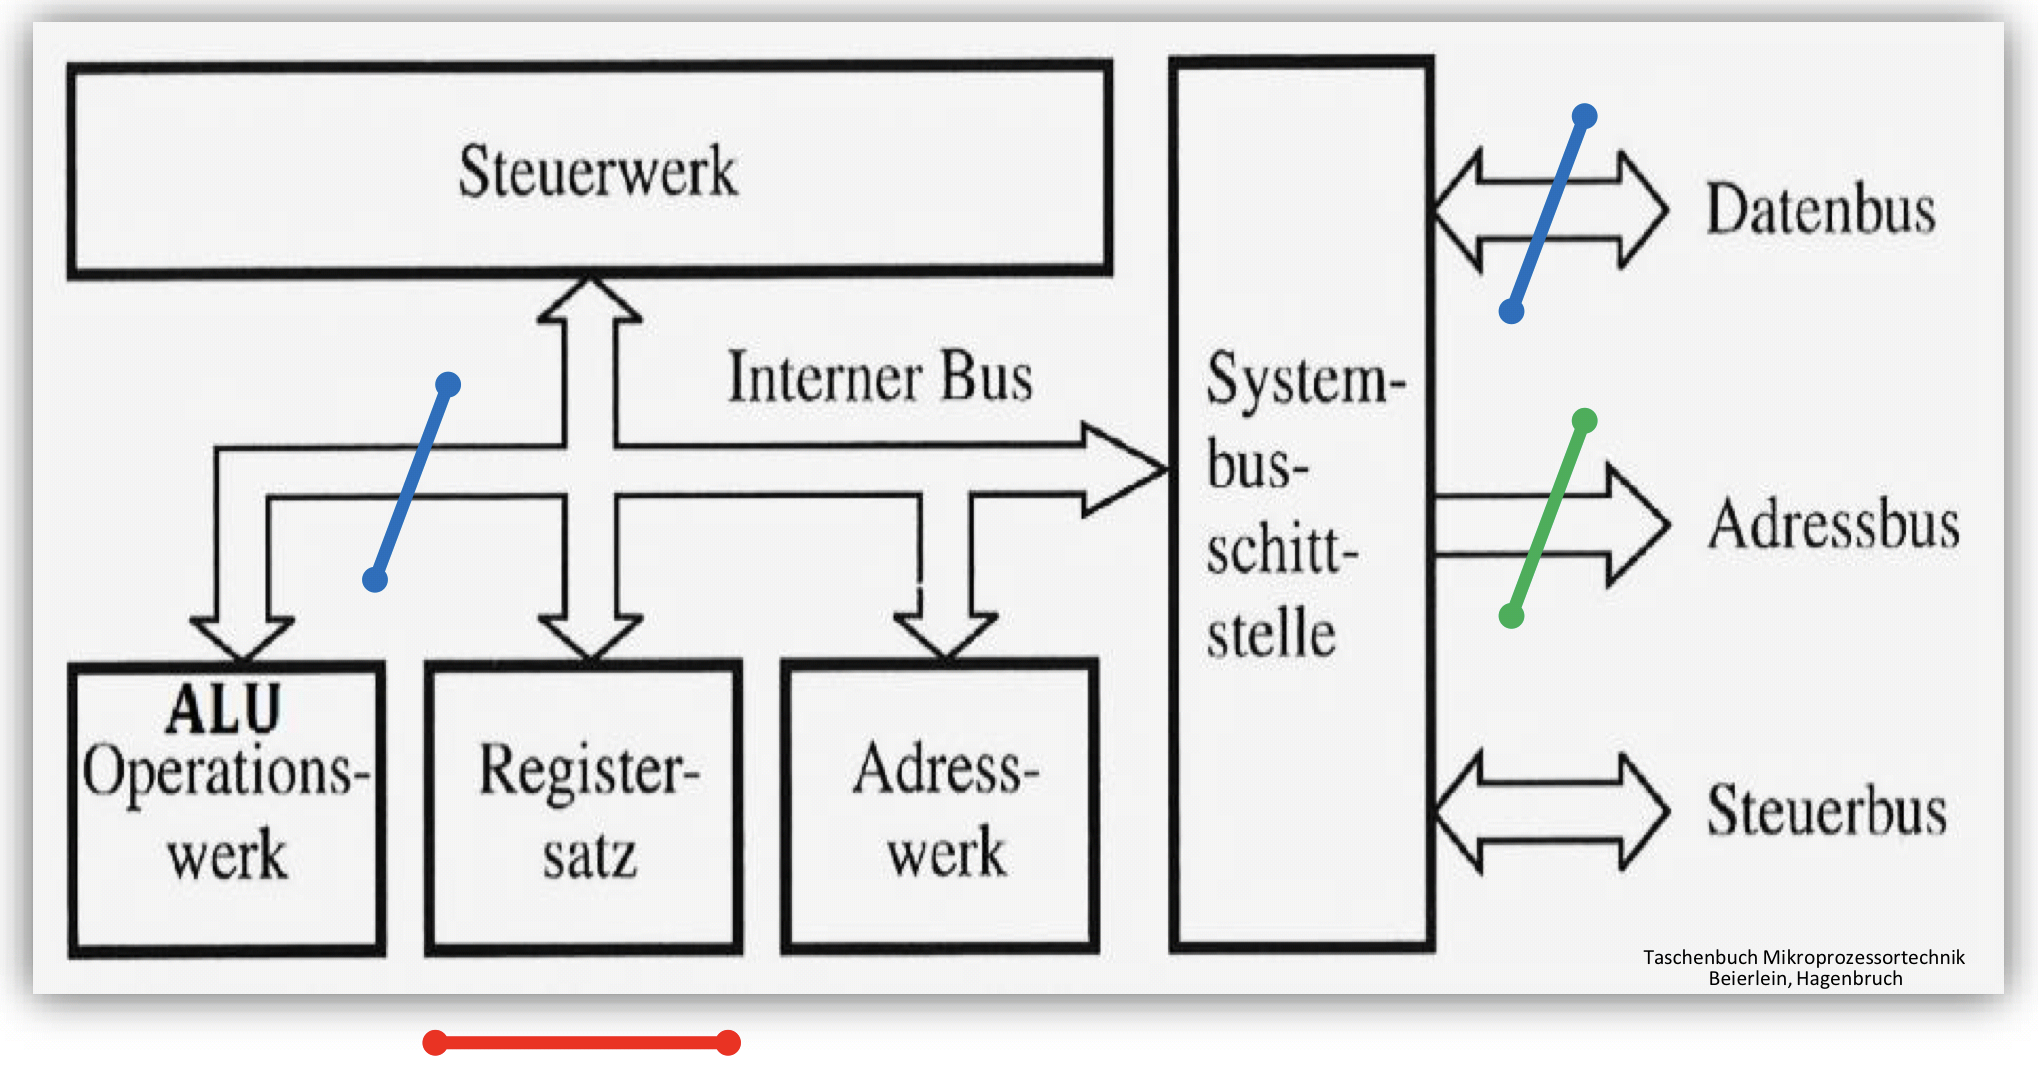
\includegraphics[width = 8cm]{pics/Komponenten-Mikroprozessor}

\begin{minipage}[t]{9cm}
	\subsubsection{Register}
	In enger Beziehung zur CPU befinden sich mehrere sehr schnell ansprechbare Register, die in ihrer Gesamtheit als Registersatz bezeichnet werden.\\
	Es wird mindestens ein \textbf{Akkumulator} ben"otigt (Universal-Register), der PicoBlaze hat sechzehn 8-Bit Universal-Register. Zudem hat der PicoBlaze sechzehn Adress-Register und auch noch Register wie Befehlsz"ahler(Program Counter, PC), Status-Register, Flags, Stackpointer usw.
\end{minipage}
%
\begin{minipage}{0.5cm}
	\ \
\end{minipage}
%
\begin{minipage}[t]{9cm}
	\subsubsection{Flags}
	Flags sind Attribute, welche das Ergebnis einer ALU-Operation zus"atzlich kennzeichnen. Die Flags befinden sich in einem Flag-Register und werden gesetzt wenn die Flag-Bedingung infolge einer ALU-Operation erf"ullt ist.
	
	Es gibt das \textbf{Zero-Flag}(Z), das \textbf{Carry-Flag}(C), das \textbf{Overflow-Flag}(V) und das \textbf{Negative-Flag}(N), eventuell gibt es noch weitere.
\end{minipage}

\begin{minipage}[t]{9cm}
	\subsubsection{ALU, Arithmetik-Logic Unit}
	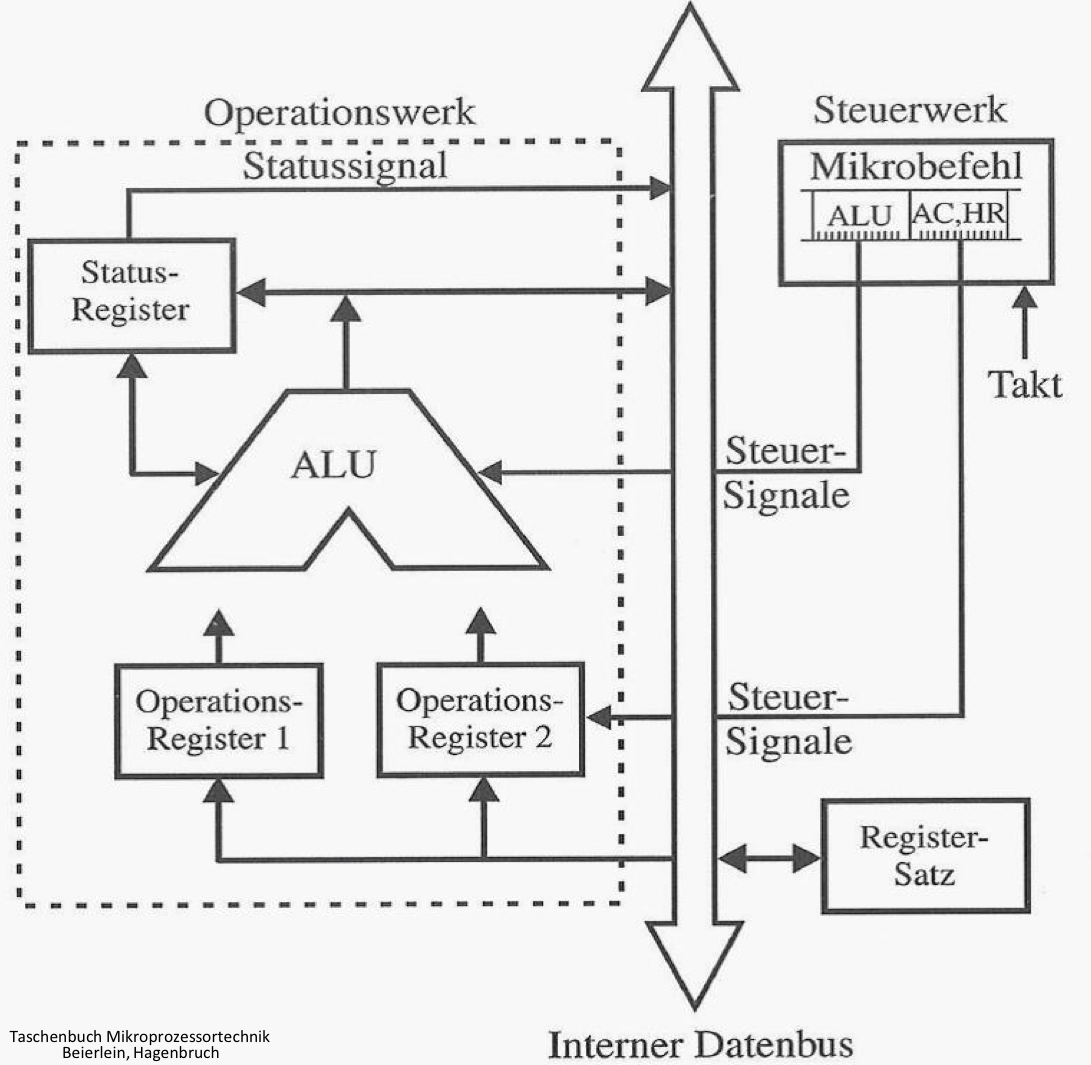
\includegraphics[width=6cm]{pics/ALU}\\
	Die \textbf{Arithmetic Logic Unit} "ubernimmt im Mikroprozessor die Datenverarbeitungsfunktion. Sie kann arithmetische Operationen wie \textbf{Addition, Subtraktion, Vergleiche}, logische Verkn"upfungen wie \textbf{AND, OR, XOR} und Verschiebungen von Bitstellen also \textbf{SHIFT} und \textbf{ROTATE}. Die Gr"osse der ALU-Operanden definiert die Einstufung des $\mu P$ als 8-, 16-, 32- oder 64-Mikroprozessor.
	
	\subsubsection{Systembus}
	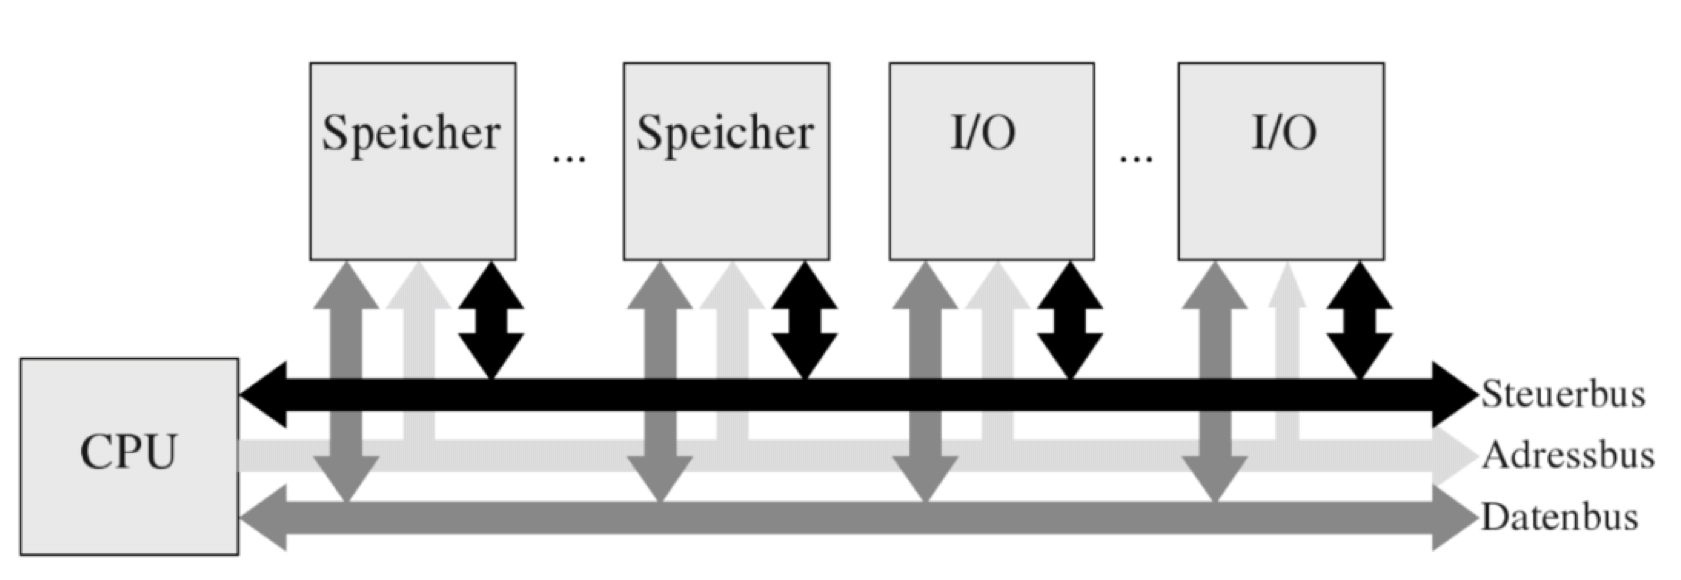
\includegraphics[width=7cm]{pics/Systembus}\\
	Die Teilbusse Datenbus, Adressbus und Steuerbus bilden gemeinsam den Systembus des Mikrocontrollers. Die Bus-Spezifikation besteht aus Funktionsbeschreibung und Operationen, elektrische Eigenschaften, zeitliche Eigenschaften usw..

\end{minipage}
%
\begin{minipage}{0.5cm}
	\ \
\end{minipage}
%
\begin{minipage}[t]{9cm}
	\subsubsection{Steuerwerk, Control Unit}
	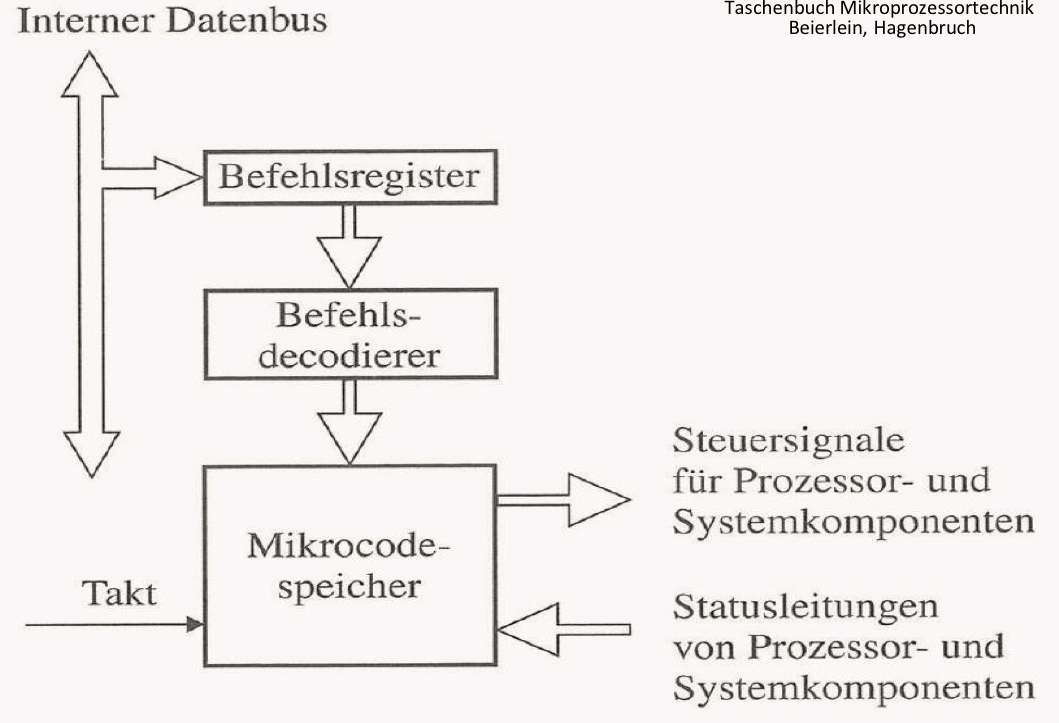
\includegraphics[width=7cm]{pics/Befehlsregister}
	
	Das \textbf{Steuerwerk} steuert im Zeitraster des Taktsignals alle Abl"aufe innerhalb der CPU und den gesamten Informationsaustausch auf dem internen Bus, sowie auf dem Datenbus zwischen CPU und Speicher- bzw. Eingabe-/Ausgabe-Einheiten.
	
	Aufgaben des Steuerwerkes:
	\begin{itemize}
		\item Steuerung aller prozessinternen Abl"aufe
		\item Bereitstellung von Adress-Informationen
		\item Steuerung der Abl"aufe auf dem Systembus
	\end{itemize}

	Der \textbf{Befehlsz"ahler (Program Counter, PC)} enth"alt stets die aktuelle Befehlsadresse. Bei jedem Befehlswortzugriff wird der PC um die entsprechende Befehlsgr"osse inkrementiert.
	
	\subsubsection{Adresswerk, Address Unit}
	Das Adresswerk berechnet nach den Vorschriften des Steuerwerks die Adresse der geforderten Operanden oder auszuf"uhrenden Befehle im Speicher.
\end{minipage}

\subsection{Ausgew"ahlte Funktionsprinzipien}
F"ur die Beschreibung der Funktionsprinzipen wird ein \textbf{Von-Neumann-Rechner} verwendet.

\begin{minipage}[t]{8cm}
	\subsubsection{Befehlsabarbeitung}
	Der \textbf{Instruction Code} wird in einer Endlos-Schleife ausgef"uhrt.\\
	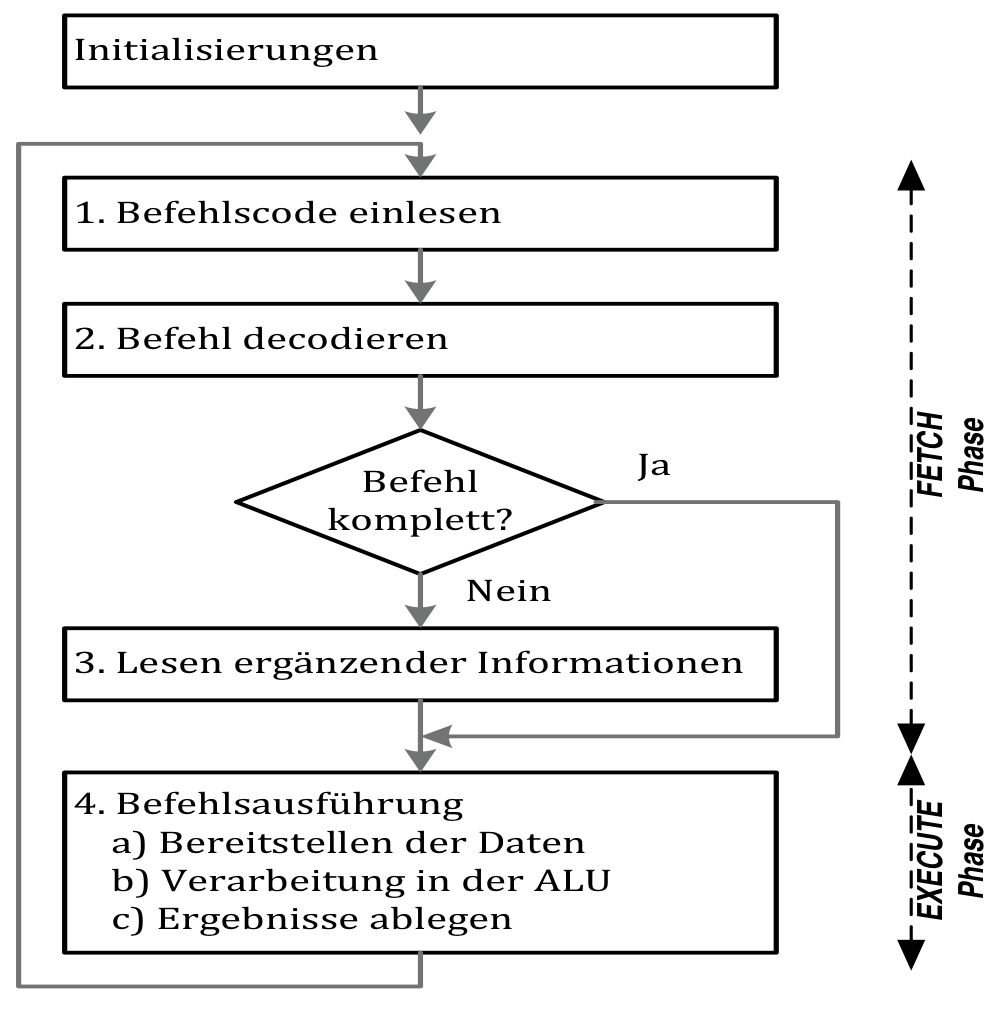
\includegraphics[width=5cm]{pics/Befehlablauf}
\end{minipage}
%
\begin{minipage}{0.5cm}
	\ \
\end{minipage}
%
\begin{minipage}[t]{10cm}
	\subsubsection{Bussteuerung}
	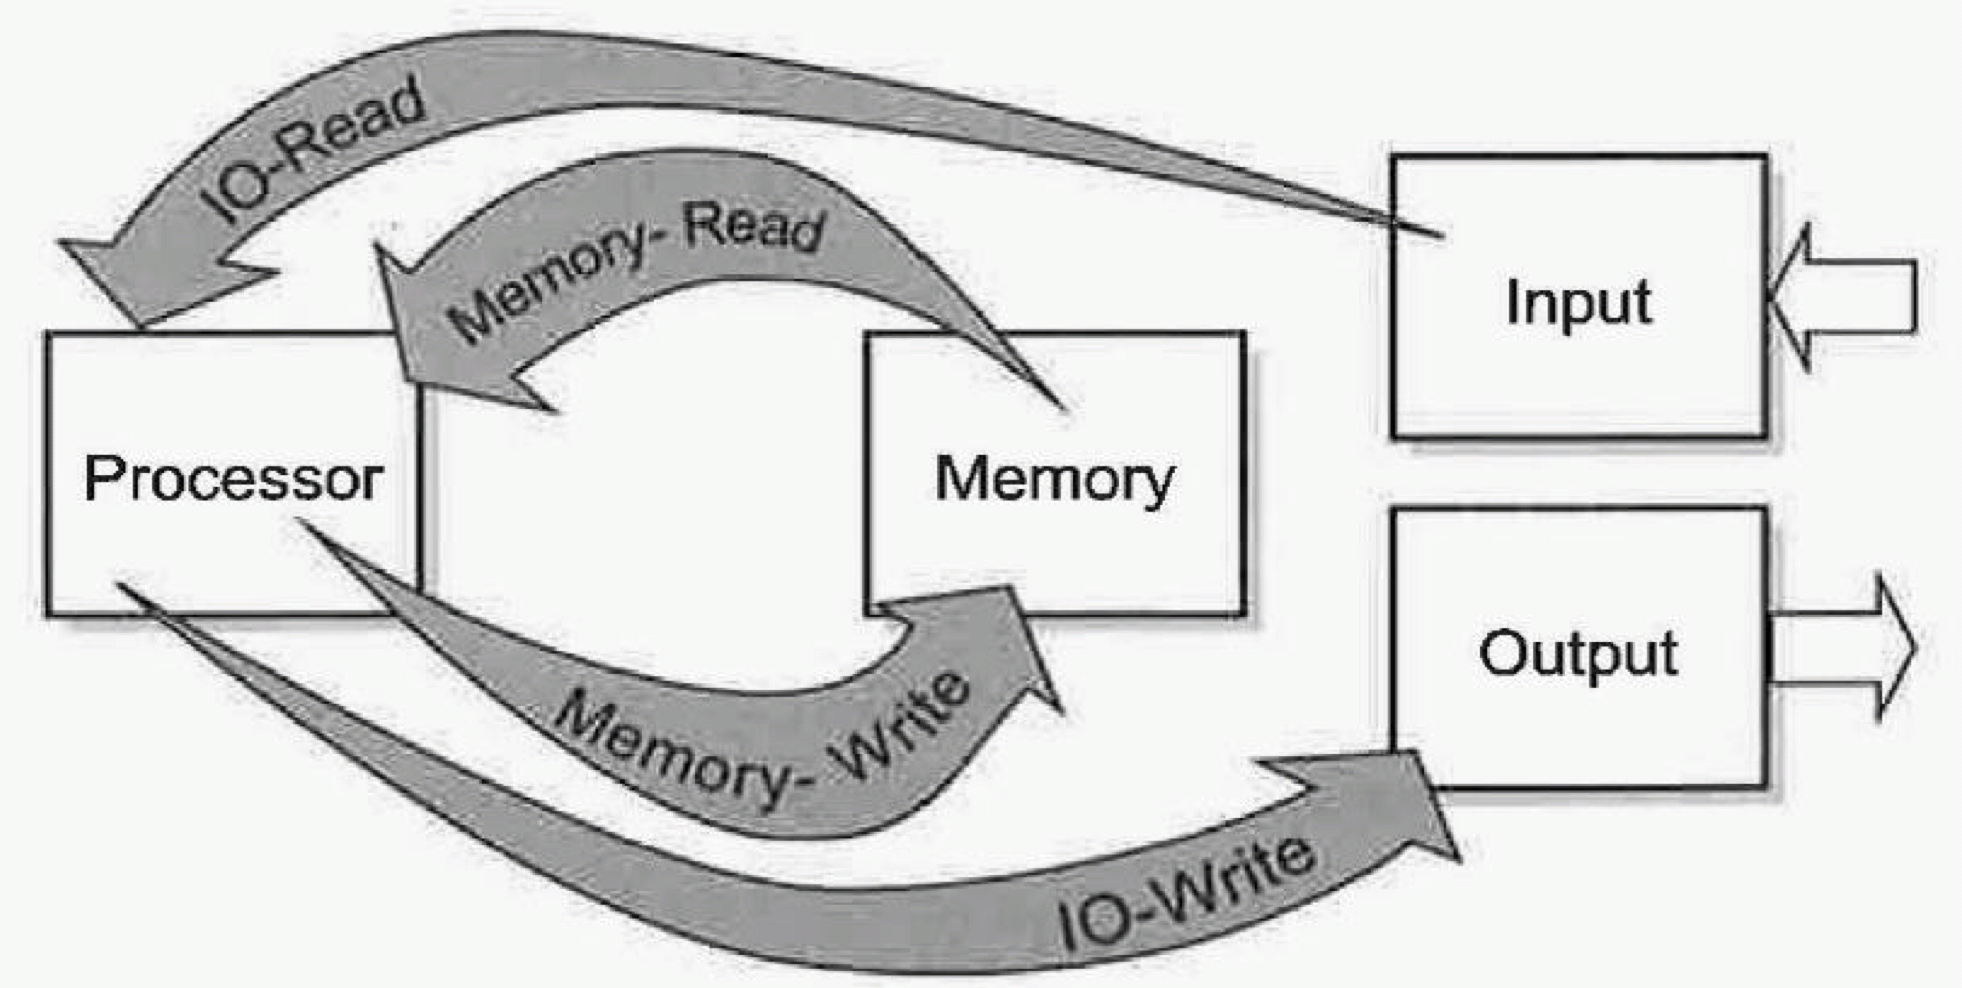
\includegraphics[width=6cm]{pics/Bus-Operationen}\\
	Man sieht, dass alle Transfers "uber den Prozessor gehen, eine Ausnahme bilden Peripherien mit DMA-Funktionalit"at, welche die Master-Funktion vor"ubergehend "ubernehmen k"onnen.
	Zudem gibt es den \textbf{asynchronen Systembus}, bei welchem mit speziellen Steuersignalen die Synchronasitation hergestellt wird und den \textbf{Synchronen Systembus}, bei welchem mit einem gemeinsamen Bustakt synchronisiert wird.
\end{minipage}
	
\begin{minipage}[t]{8cm}
	\subsubsection{Ankopplung von Eingabe und Ausgabe-Einheiten}
	Damit Peripherien an einen Mikroprozessor angeschlossen werden k"onnen ben"otigt es Interface-Bausteine, welche wesentlich aus zwei Komponenten bestehen, aus der Elektronik zur Ankopplung an den Bus des Mikroprozessors und aus einer konfigurierbaren Elektronik zur Ankopplung der externen Komponenten.\\
	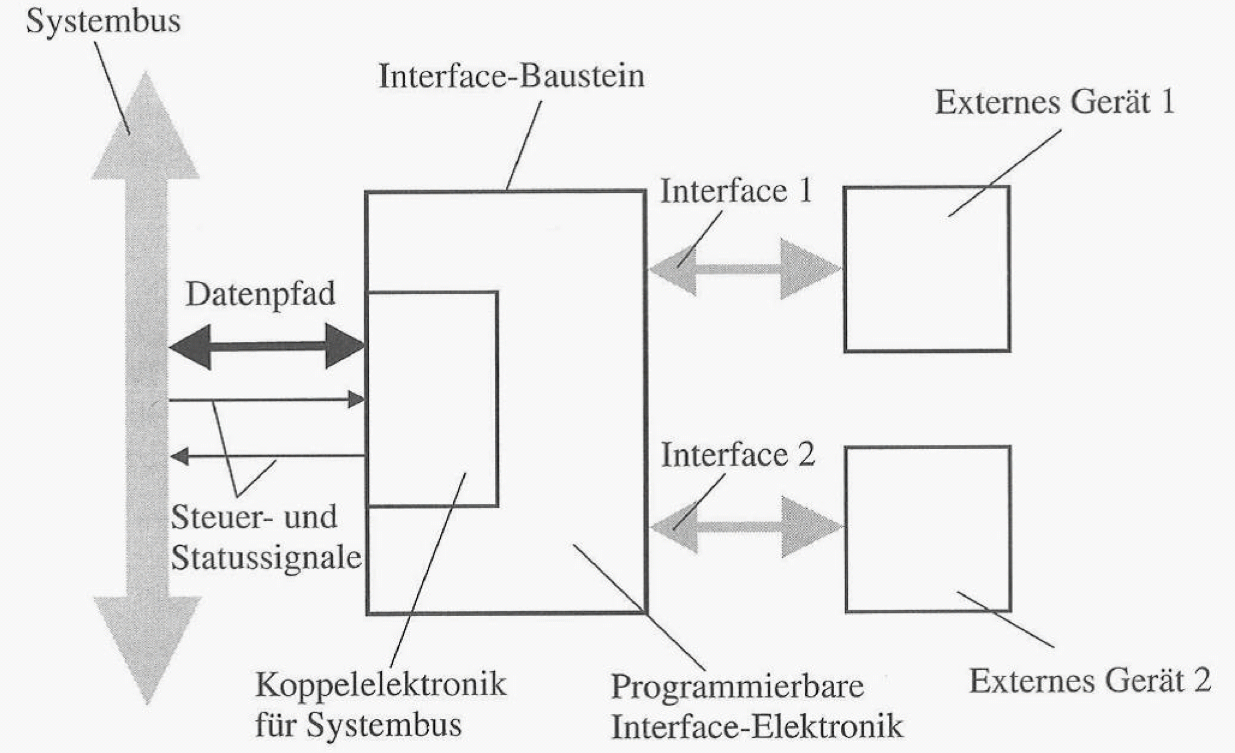
\includegraphics[width=5.5cm]{pics/Interface-Komponenten}
\end{minipage}
% 
\begin{minipage}{0.5cm}
	\ \
\end{minipage}
%
\begin{minipage}[t]{10cm}
	\subsubsection{Memory-Mapped I/O}
	Bei der Ansteuerung der Interface-Bausteine als I/O-Komponenten bieten sich zwei grunds"atzliche Konzepte an:\\
	\textbf{Isolierte Adressierung:} Separater Adressraum f"ur I/O und Speicher. Verschiedene Prozessor-Instruktionen (z.B. /MEMR, /MEMW oder /IOR, /IOW).\\
	\textbf{Memory-Mapped I/O:} Der Adressraum von I/O und Speicher ist nicht getrennt. Ansprechung durch dieselben Prozessor-Instruktionen.\\
	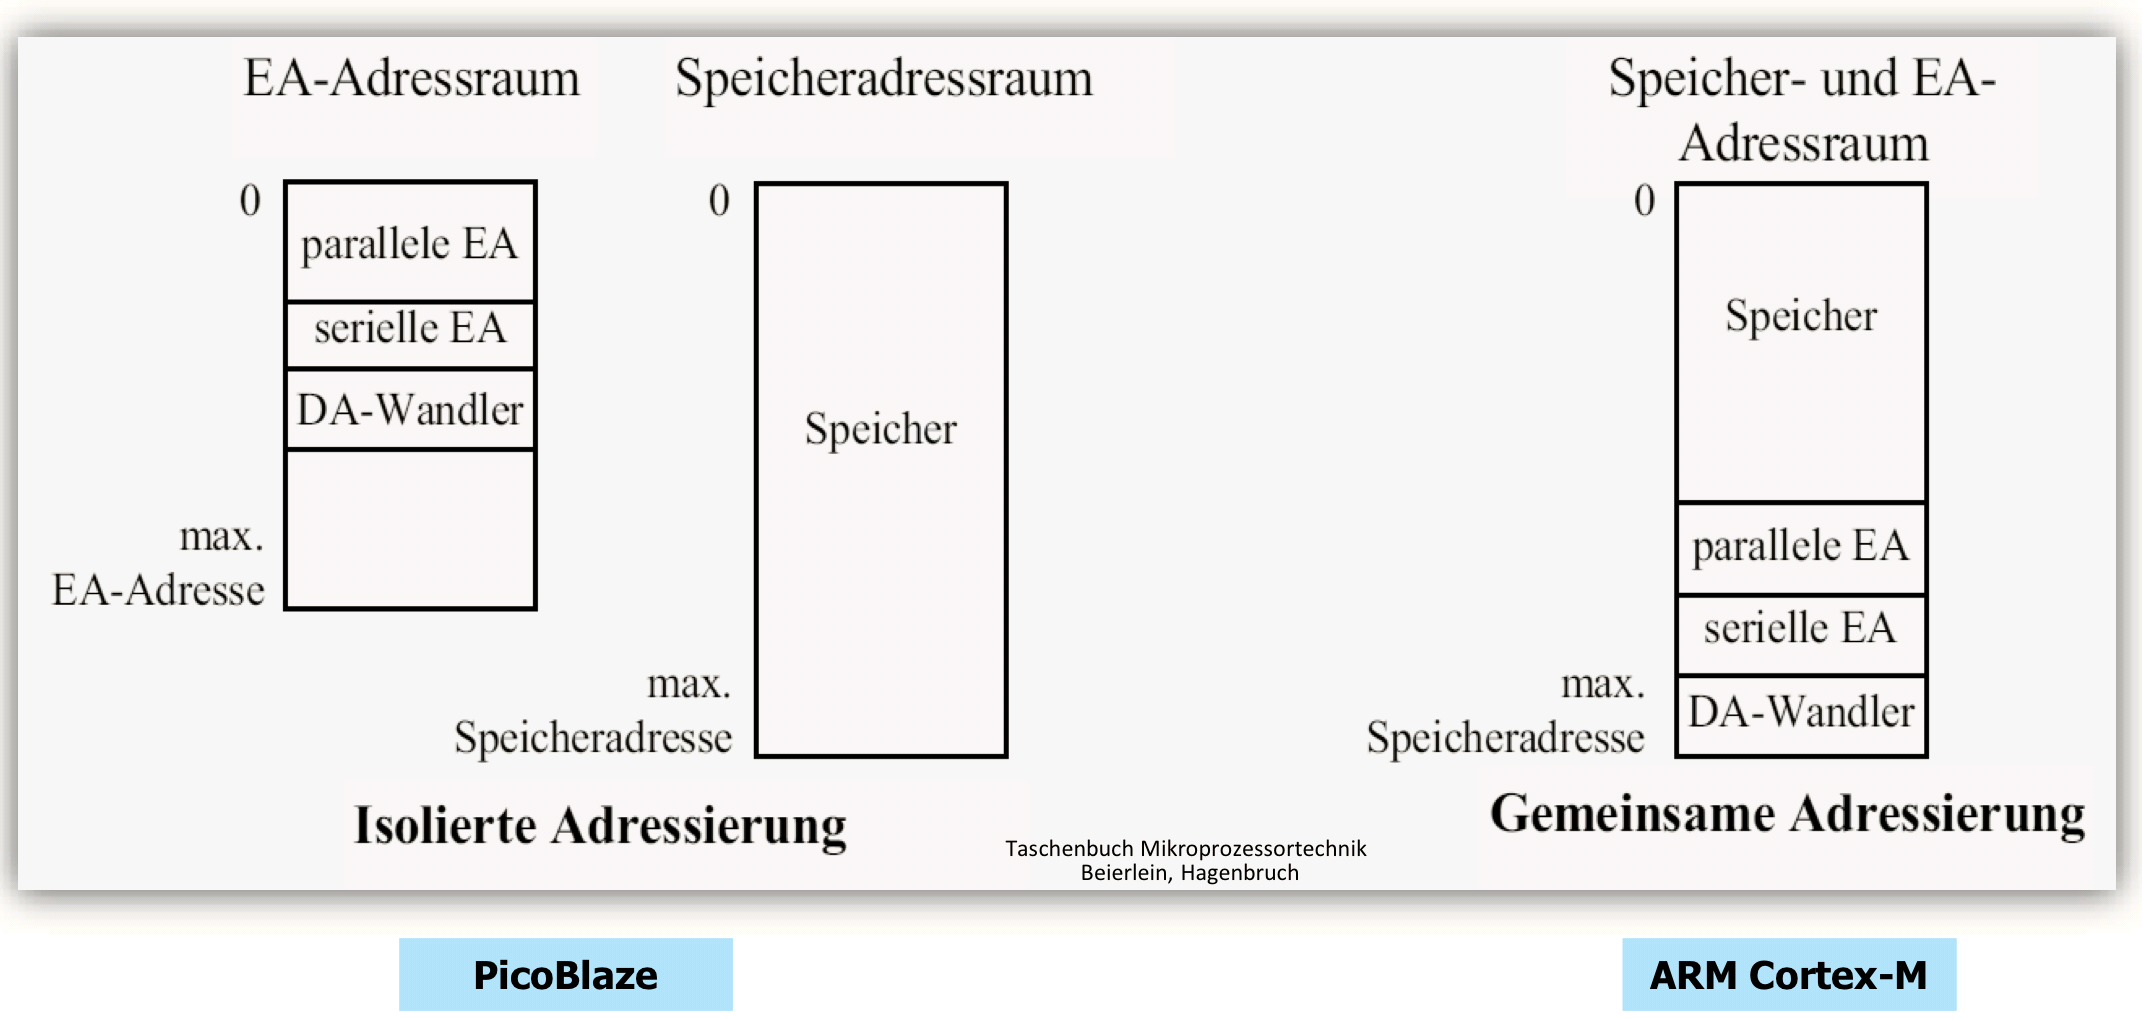
\includegraphics[width=7.5cm]{pics/Adressbereich}
\end{minipage}

\begin{minipage}[t]{8cm}
	\subsubsection{Stack-Funktion}
	Der \textbf{Stapelspeicher (Stack)}, ist ein reservierter Speicherbereich, der mittels Stack Pointer, SP, nach dem Last-In-First-Out-Prinzip (LIFO) verwaltet wird. Mit dem \textbf{PUSH} Befehl k"onnen Daten-Elemente dem Stack hinzugef"ugt werden und mit dem \textbf{POP} Befehl k"onnen sie wieder entnommen werden.\\
	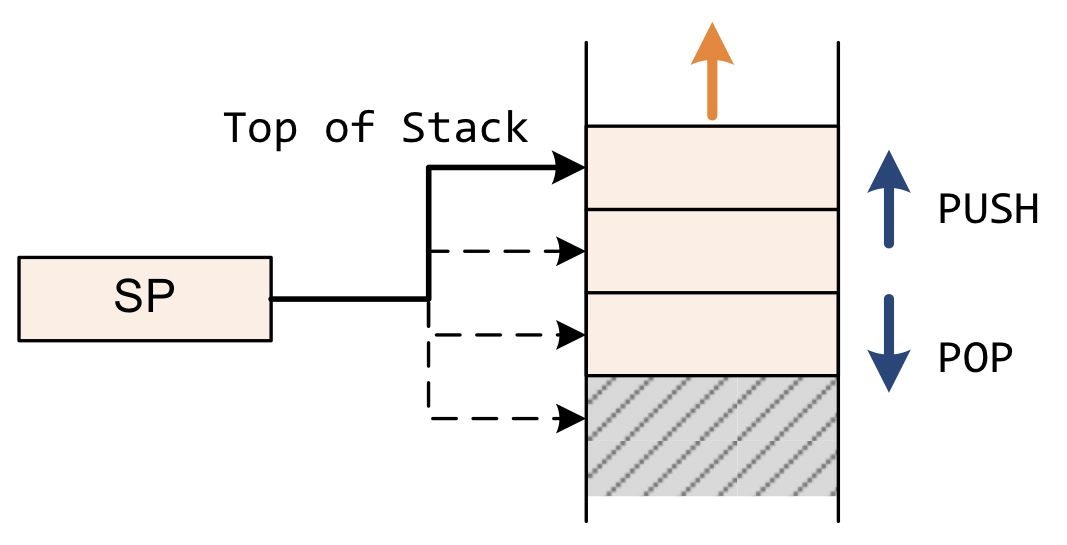
\includegraphics[width=5cm]{pics/Stack-Operationen}
\end{minipage}
%
\begin{minipage}{0.5cm}
	\ \
\end{minipage}
%
\begin{minipage}[t]{10cm}
	\subsubsection{Polling vs. Interrupt-Steuerung}
	Beim \textbf{Polling}-Verfahren wird per Programm immer kontrolliert wie die Status-Informationen aussehen und so festgestellt ob Daten von Eingabe-Einheiten eingelesen oder an Ausgabe-Einheiten ausgegeben werden k"onnen.\\
	Beim \textbf{Interrupt}-Verfahren k"onnen Ein-/Ausgabe-Einheiten eine Bedienungsanforderung per Interrupt-Request anmelden. Diese trifft asynchron ein und der Mikroprozessor entscheidet "uber den Ausf"uhrungszeitpunkt der Interrupt-Service-Routine (ISR).
		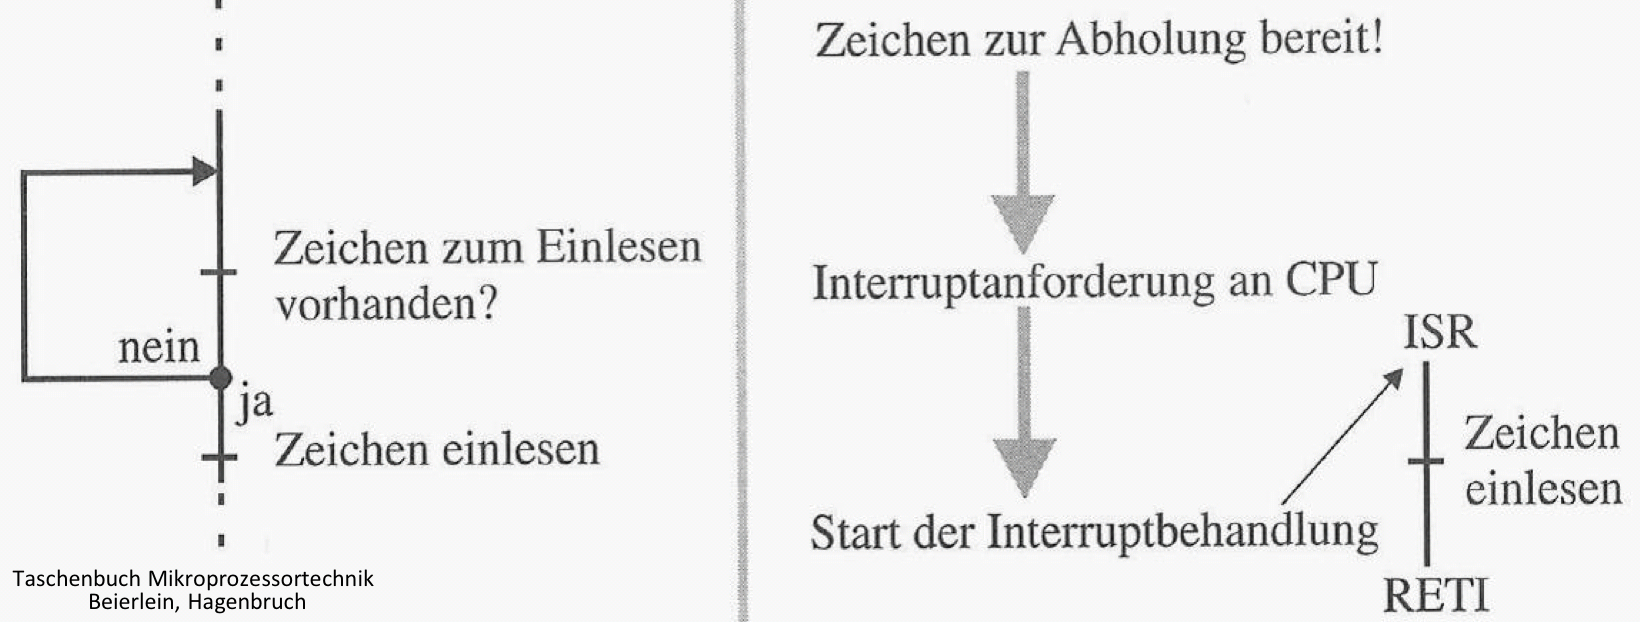
\includegraphics[width=7cm]{pics/Interrupt-operationen}
\end{minipage}

\subsection{Basis-Architekturen}
\begin{minipage}{9cm}
	\textbf{CISC-Prozessoren}(Complex Instruction Set Computer):\\
	Traditionelle Prozessoren sind nach dem CISC-Modell realisiert. CISC-Prozessoren besitzen in der Regel eine Befehlssatz mit vielen spezialisierten und leistungsf"ahigen Instruktionen.
\end{minipage}
%
\begin{minipage}{0.5cm}
	\ \
\end{minipage}
%
\begin{minipage}{9cm}
	\textbf{RISC-Prozessoren}(Reduced Instruction Set Computer):
	Sie besitzen einen kleinen (reduzierten) Befehlssatz (< 100 Befehle). Die Maschinenbefehle sind sehr einfach und kurz gehalten. Kompliziertere Befehle m"ussen aus mehreren einfachen Einzelbefehlen zusammengesetz werden.
\end{minipage}

